\subsection{Transversale Mercatorprojektion}
\label{sec:transmercator}
Bei der transversalen  Mercatorprojektion wird der Globus zuerst um 90$ ^\circ $ gedreht, so das der 0 Meridian zu Äquator wird. Danach wird eine normale Mercatorprojektion erstellt.\\

\begin{figure}[hbtp]
\centering
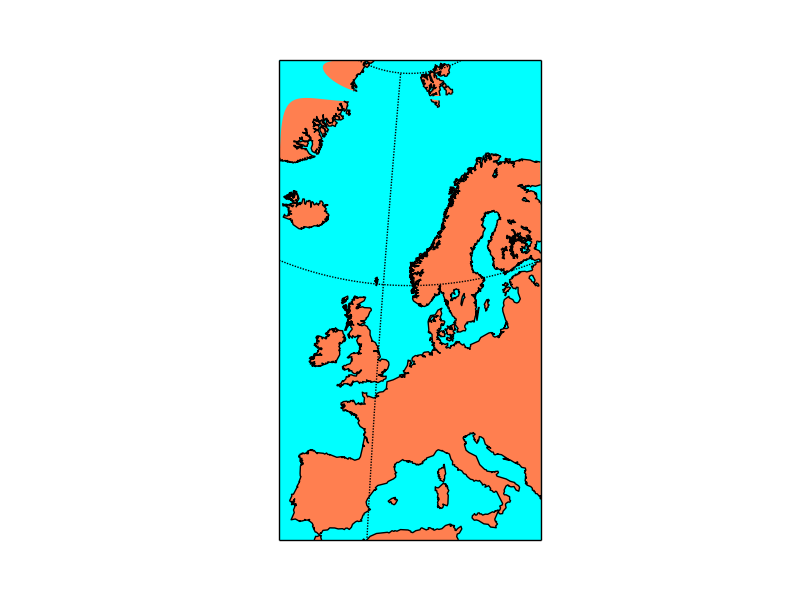
\includegraphics[scale=0.5,origin=c]{/Users/student/seminar/Kartendarstellungen/seminar/tmerc} 
\caption{Transversale Mercatorprojektion}
\end{figure}
\newpage 